
\documentclass[11pt,letterpaper]{article}

% Load some basic packages that are useful to have
% and that should be part of any LaTeX installation.
%
% be able to include figures
\usepackage{graphicx}
% get nice colors
\usepackage{xcolor}

% change default font to Palatino (looks nicer!)
\usepackage[latin1]{inputenc}
\usepackage{mathpazo}
\usepackage[T1]{fontenc}
% load some useful math symbols/fonts
\usepackage{latexsym,amsfonts,amsmath,amssymb}

% comfort package to easily set margins
\usepackage[top=1in, bottom=1in, left=1in, right=1in]{geometry}

% control some spacings
%
% spacing after a paragraph
\setlength{\parskip}{.15cm}
% indentation at the top of a new paragraph
\setlength{\parindent}{0.0cm}


\begin{document}

\begin{center}
\Large
Ay190 -- Worksheet 13\\
Anthony Alvarez\\
Date: February 25, 2014
\end{center}

\section{N-body Simulation}

We first begin by implementing RK4 scheme for n-body simulation that accounts
 for gravitational interactions between all n objects. We also make
a function that calculates the total energy of the system given a 
state vector. 

\subsection{Sun and Earth System}

When running this simulation on the Sun and Earth system we find that the Earth's
orbit remains bound with constant energy $-2.64\ 10^{40} erg$. We also find that
the Earth's orbital radius changes slighlty thought the year, as it should, but
it always comes back to the same value after a year. Our simulation doesn't
seem to be leaking or gaining energy as the total energy in the system is
very constant. Additionally, smaller stepsizes yield smaller errors as we 
would expect ~\ref{fig:phi}. Lower resolutions seem to have increasing errors while the 
highest resolution I ran had relatively constant error. 

\begin{figure}[bth]
\centering
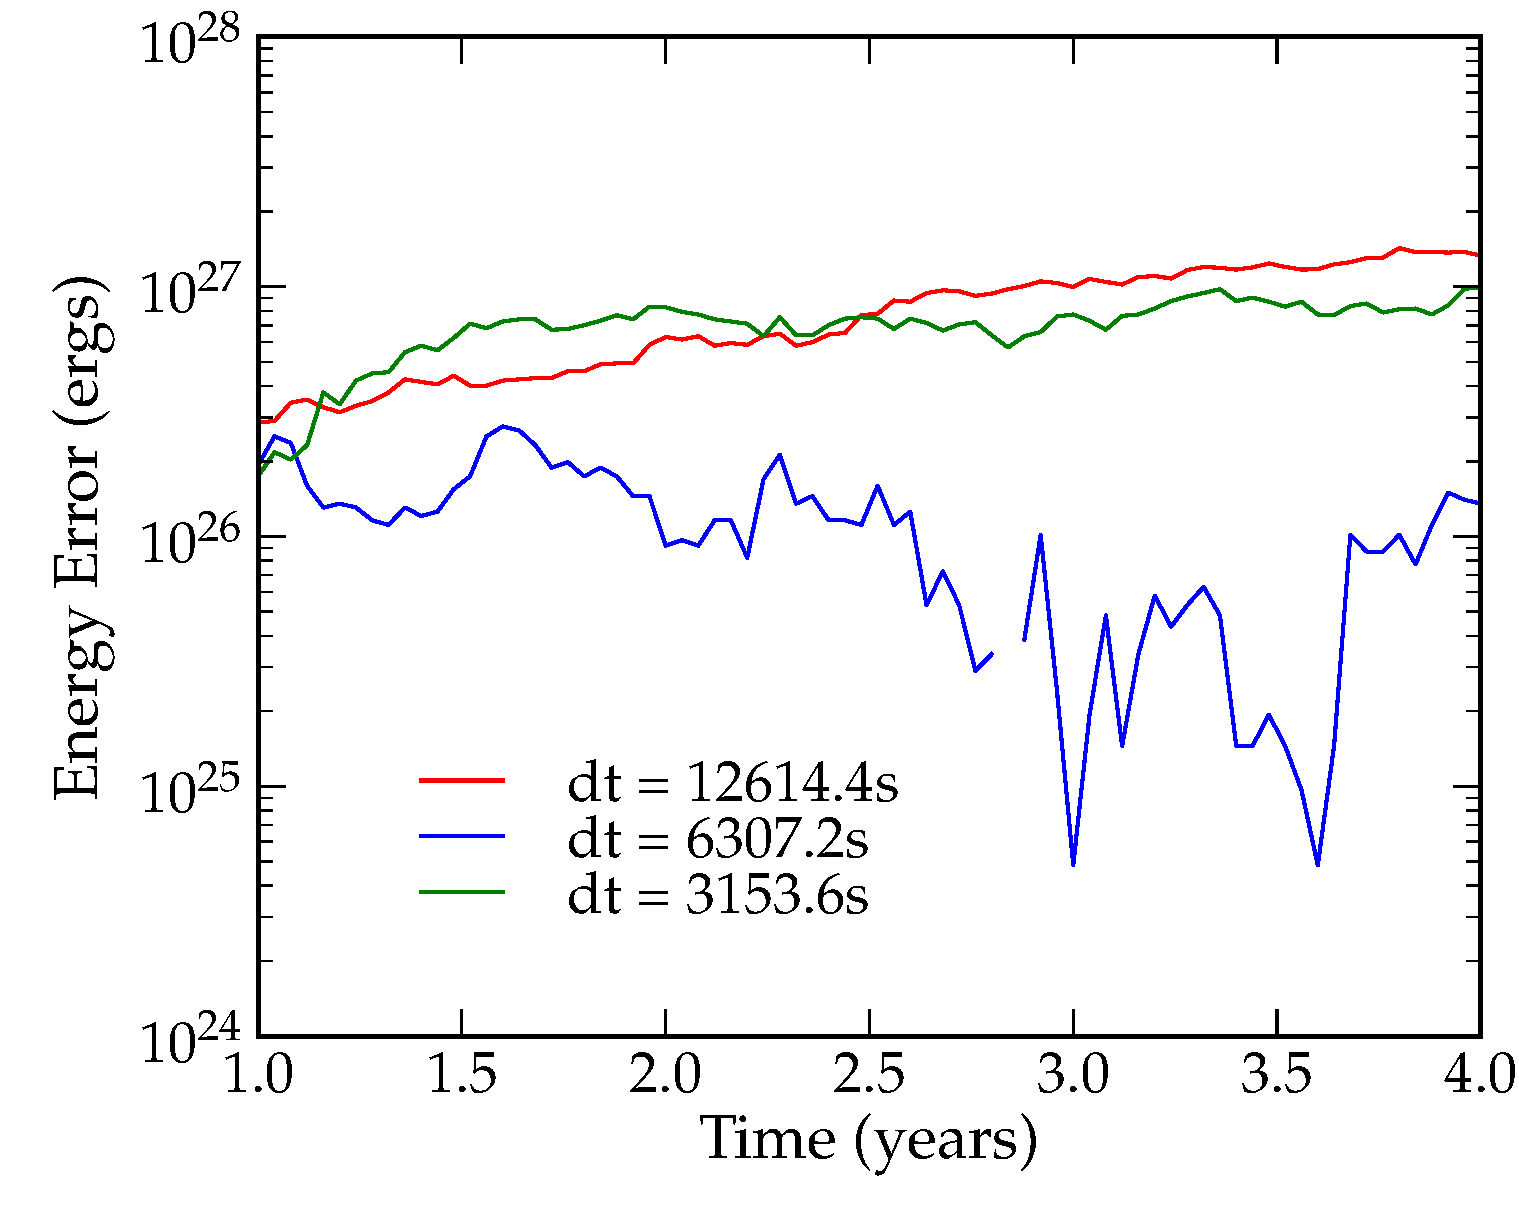
\includegraphics[width=0.5\textwidth]{3.pdf}
\caption{Energy Error for Earth Sun System.}
\label{fig:phi}
\end{figure}

\subsection{Central Black Hole System}

For the central black hole system we simulated first for 10 years just to make 
sure that the simulation was working correctly. We notice that at around 5 years
there is a large spike in the error ~\ref{fig:4a}. This is caused by a star
coming very close to the central black hole, where we would expect large 
derivatives and inaccurate numerical integration. 

\begin{figure}[bth]
\centering
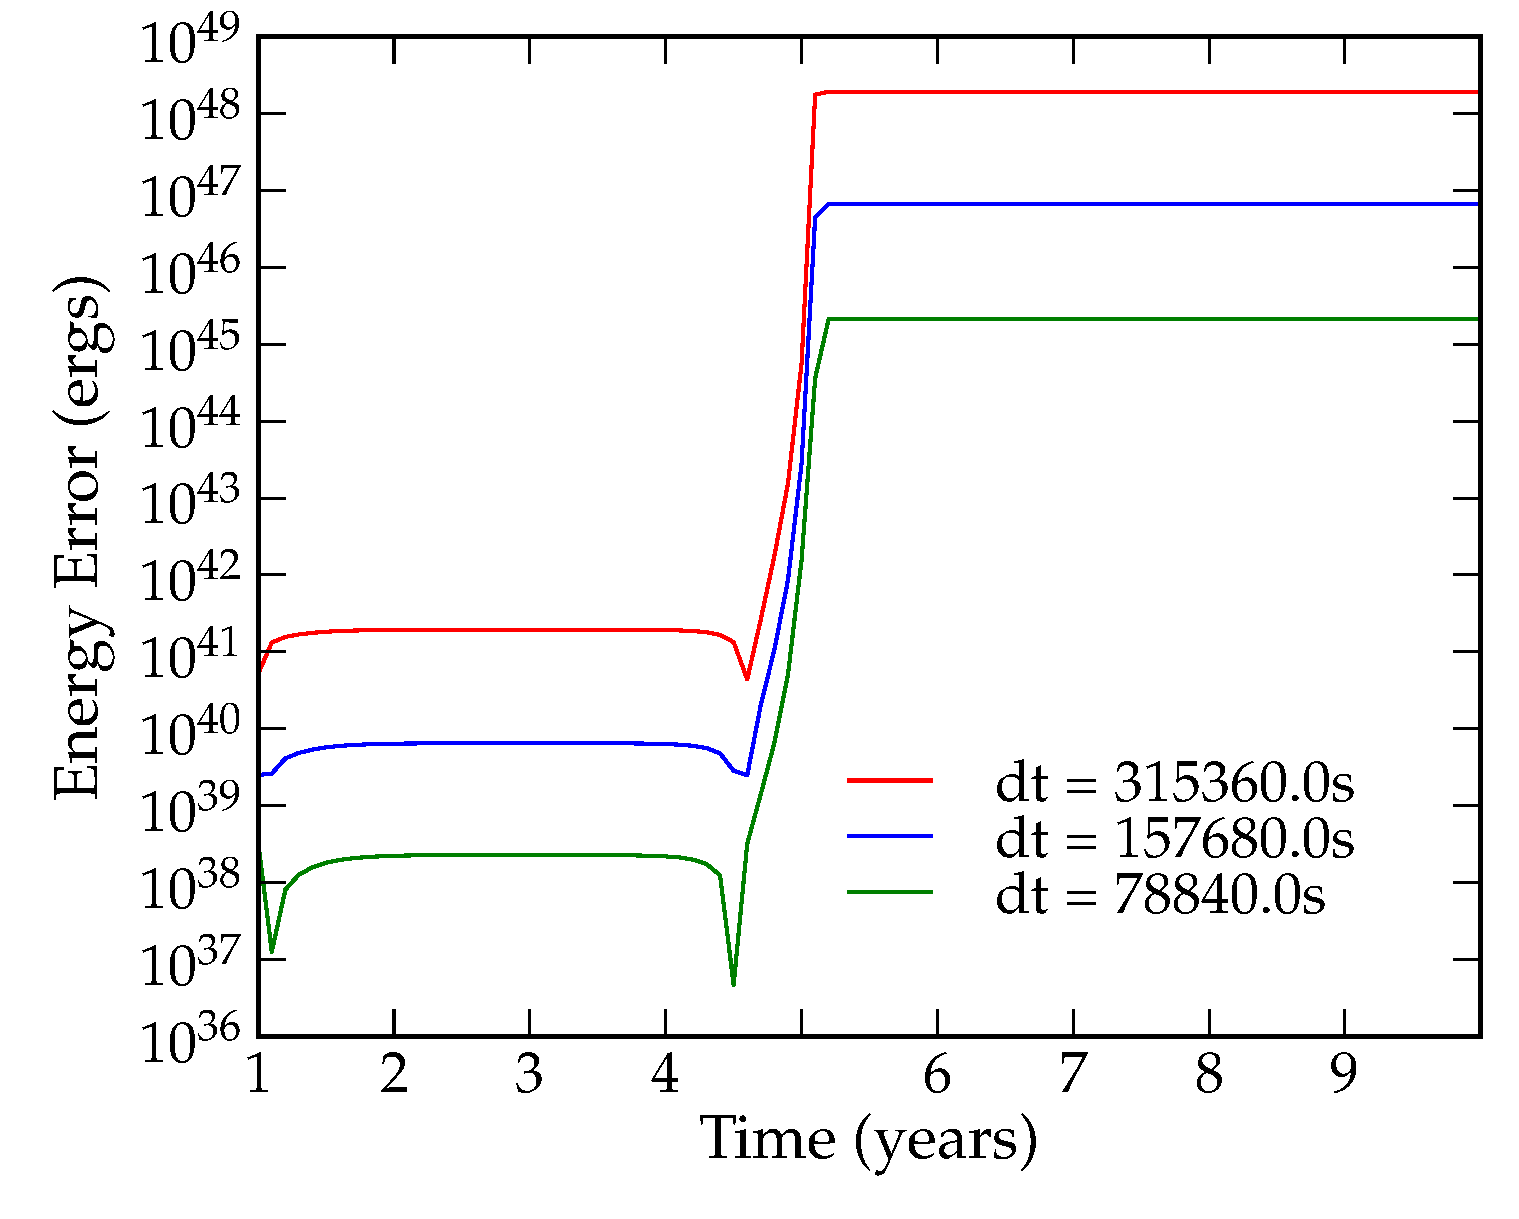
\includegraphics[width=0.5\textwidth]{4a.pdf}
\caption{Energy Error for Central black hole system}
\label{fig:4a}
\end{figure}

We isolated just the first 4 years before the bumb to see if there were effects
we couldn't see ~\ref{fig:4b}. We did not notice anything out of the ordinary.

\begin{figure}[bth]
\centering
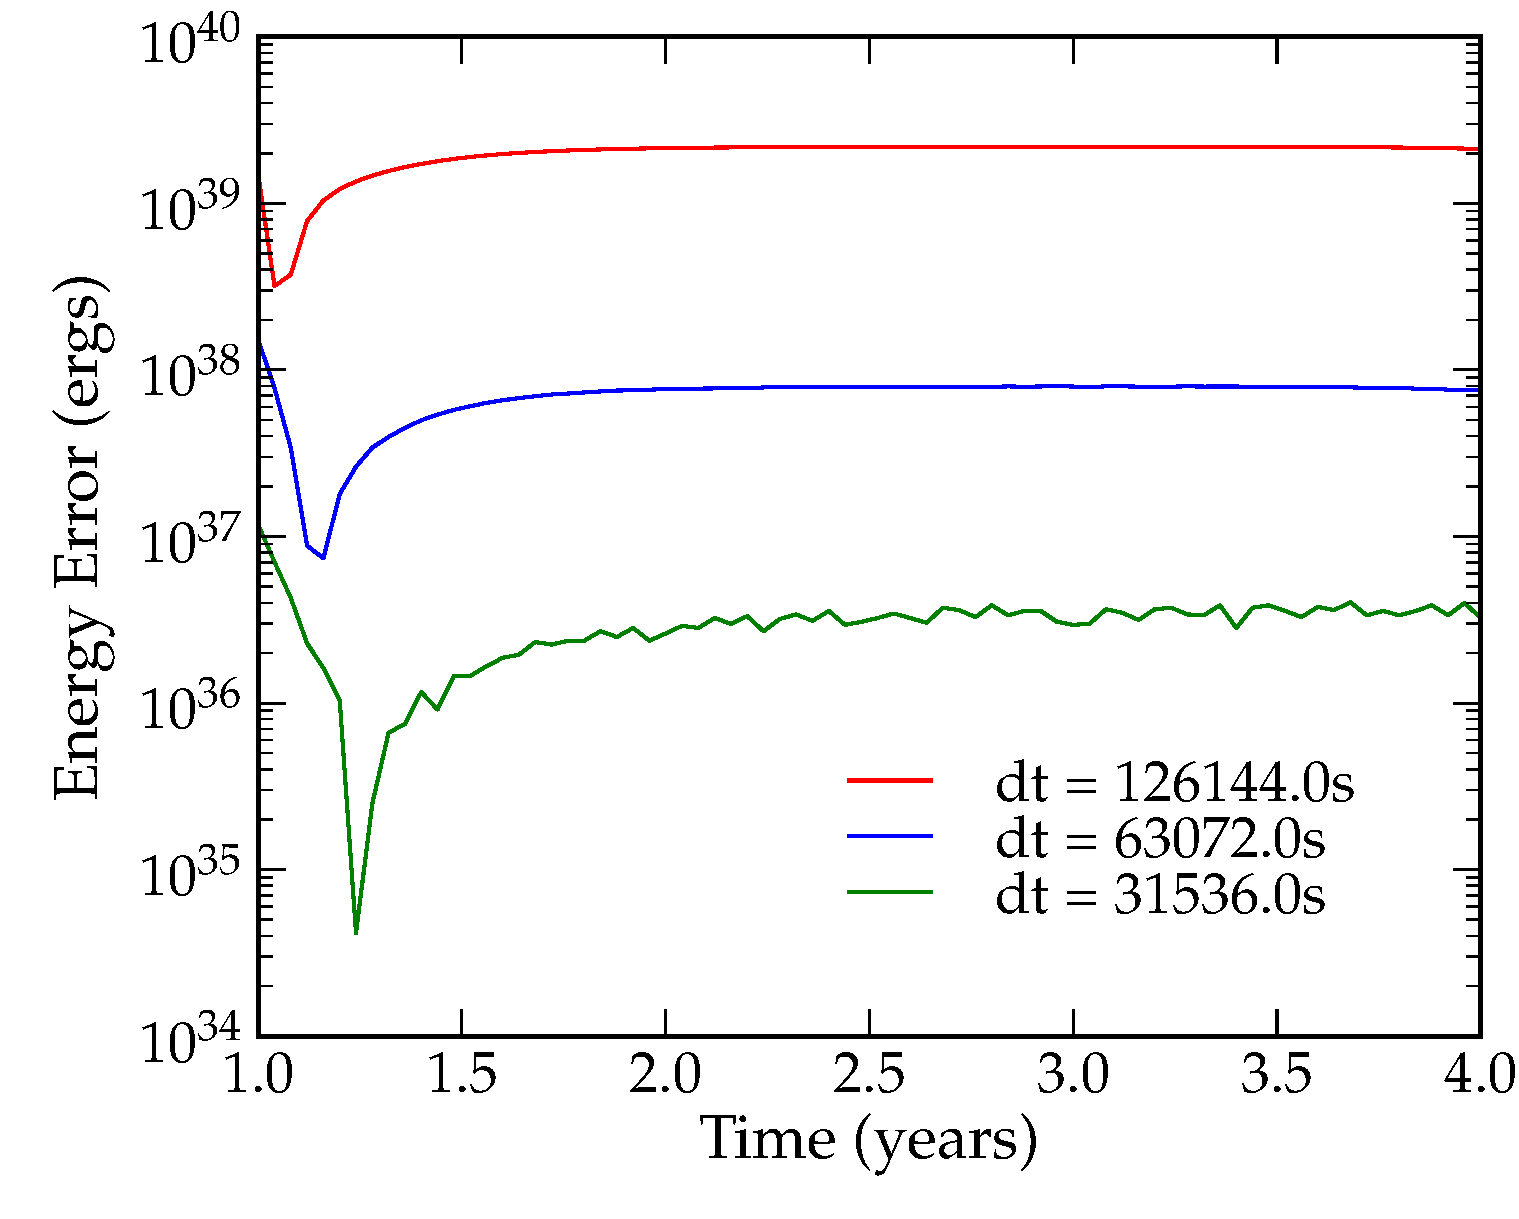
\includegraphics[width=0.5\textwidth]{4b.pdf}
\caption{Energy Error for Central black hole system}
\label{fig:4b}
\end{figure}

We then ran the population of stars for 100 years and noted that for low
resolutions the system becomes unbounded after 30 years. We increased the 
resolution to 10000 points for 100 years and then compared the final 
positions to the data obtained from \begin{verbatim}
http://astro.uchicago.edu/cosmus/projects/UCLS_GCG/ \end{verbatim}. 
We found that the positions
we calculated (-0.1456,,0.067,-0.112) were vastly different than the final 
position calculated by uChicago (0.218,-0.452,-0.234). This
is expected as small numerical errors, even rounding will compound over many 
itterations of code. 

\end{document}




